\section{Variació mitjana d'una funció en un interval}

Donada una funció $y = f(x)$, s'anomena \textbf{variació mitjana de la funció} en l'interval $[x_1, x_2]$ el valor numèric del quocient:

\begin{equation*}
\frac{f(x_2) - f(x_1)}{x_2 - x_1} = \frac{\Delta f(x)}{\Delta x} = \frac{\Delta y}{\Delta x}
\end{equation*}

\begin{itemize}
\item Si $y = f(x)$ és creixent a l'interval $[x_1, x_2]$, la seva variació mitjana és \textbf{positiva}.
\item Si $y = f(x)$ és decreixent a l'interval $[x_1, x_2]$, la seva variació mitjana és \textbf{negativa}.
\end{itemize}

\section{Variació d'una funció en un punt}

La variació d'una funció $f$ en el punt $x_0$ es defineix com el límit:

\begin{equation*}
\lim_{x\to x_0} \frac{f(x) - f(x_0)}{x - x_0}
\end{equation*}

\section{Derivada d'una funció en un punt}

\textbf{Definició:} La \textbf{derivada} d'una funció $f$ en el punt $x_0$ és

\begin{equation}
f'(x_0) = \lim_{x\to x_0} \frac{f(x) - f(x_0)}{x - x_0}
\end{equation}

sempre que aquest límit existeixi i sigui finit.

A partir d'aquesta definició es dedueixen els criteris de creixement local:

\begin{itemize}
\item Si $f'(x_0) > 0$, la funció és \textbf{creixent} en $x = x_0$.
\item Si $f'(x_0) < 0$, la funció és \textbf{decreixent} en $x = x_0$.
\item Si $f'(x_0) = 0$, la funció quasi no varia per a valors de $x$ pròxims a $x_0$.
\end{itemize}

\section{Creixement i decreixement. Punts estacionaris}

La definició de derivada d'una funció $y = f(x)$ en un punt $x = x_0$ permet afirmar que:

\begin{itemize}
\item Si $f'(x_0) > 0$, la funció és \textbf{creixent} en aquest punt.
\item Si $f'(x_0) < 0$, la funció és \textbf{decreixent} en aquest punt.
\item Si $f'(x_0) = 0$, la funció presenta en $x_0$ un \textbf{màxim}, un \textbf{mínim} o un \textbf{punt d'inflexió} de tangent horitzontal.
\end{itemize}

La figura següent il\textperiodcentered{}lustra aquests conceptes sobre una corba representativa:

\begin{figure}[!htbp]
\centering
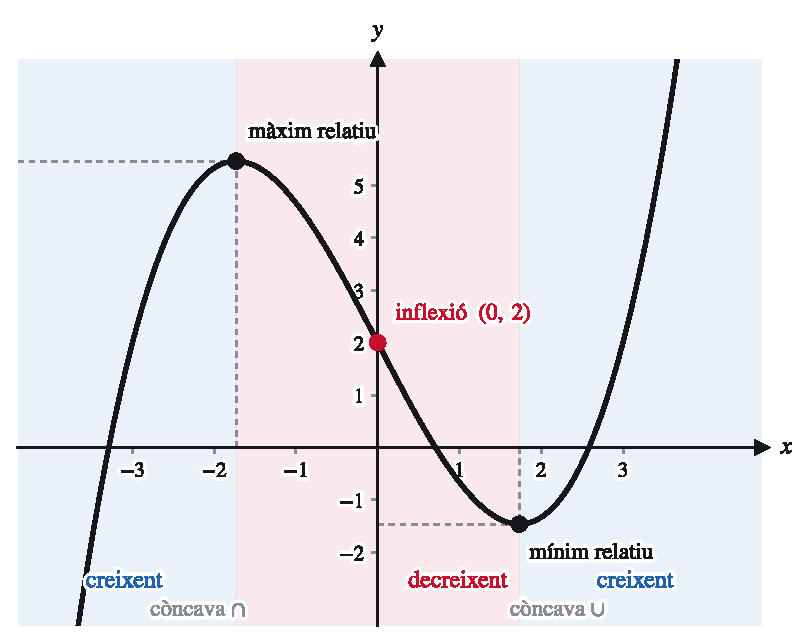
\includegraphics[width=389pt]{fig/m01_f01.pdf}
\caption{Representació dels conceptes de creixement, decreixement, màxim i mínim relatius, punt d'inflexió i concavitat per a $f(x) = \frac{x^3}{3} - 3x + 2$.}
\end{figure}

\section{Derivabilitat d'una funció en un punt}

\textbf{Definició:} Diem que una funció $y = f(x)$ és \textbf{derivable} en el punt $x = x_0$ si existeix el nombre $f'(x_0)$, derivada de la funció en aquest punt.

\textbf{Propietat:} Perquè una funció $y = f(x)$ sigui derivable en $x = x_0$, necessàriament ha de ser \textbf{contínua} en aquest punt. Si una funció presenta qualsevol tipus de discontinuïtat en $x = x_0$, no existeix $f'(x_0)$.

\section{Funció derivada}

La definició alternativa de la derivada, equivalent a la de l'apartat 3, és:

\begin{equation*}
f'(x_0) = \lim_{h\to 0} \frac{f(x_0 + h) - f(x_0)}{h}
\end{equation*}

Les regles pràctiques bàsiques de derivació, conegudes del curs anterior, són:

\begin{itemize}
\item Funció constant: $f(x) = k \Rightarrow f'(x) = 0$
\item Funció potencial: $f(x) = x^n \Rightarrow f'(x) = n \cdot x^{n-1}$, $\; n \in \mathbb{N}$
\item Funció suma: $f(x) = p(x) + q(x) \Rightarrow f'(x) = p'(x) + q'(x)$
\item Producte d'una constant per una funció: $f(x) = k \cdot g(x) \Rightarrow f'(x) = k \cdot g'(x)$
\end{itemize}

\section{Derivada de la funció composta. Regla de la cadena}

\textbf{Definició (Regla de la cadena):} Si $f(x) = g[u(x)]$, aleshores

\begin{equation}
f'(x) = g'[u(x)] \cdot u'(x)
\end{equation}

És a dir, per derivar una funció composta es deriva l'exterior (avaluat a l'interior) i es multiplica per la derivada de l'interior.

\section{Derivades successives}

Donada una funció derivable $f(x)$, podem trobar la seva funció derivada $f'(x)$. Moltes vegades, aquesta nova funció també és derivable. Les derivades d'ordre superior es defineixen de manera inductiva:

\begin{equation*}
f(x) \xrightarrow{\ \frac{d}{dx}\ } f'(x) \xrightarrow{\ \frac{d}{dx}\ } f''(x) \xrightarrow{\ \frac{d}{dx}\ } f'''(x) \xrightarrow{\ \frac{d}{dx}\ } \cdots \xrightarrow{\ \frac{d}{dx}\ } f^{(n)}(x)
\end{equation*}

on $f''(x)$ és la derivada segona, $f'''(x)$ la derivada tercera, i $f^{(n)}(x)$ la derivada enèsima de $f$.

Cal destacar alguns casos particulars:

\begin{itemize}
\item \textbf{Funcions polinòmiques:} per derivació successiva, qualsevol polinomi de grau $n$ s'anul\textperiodcentered{}la al derivar-lo $n + 1$ vegades.
\item \textbf{Funció exponencial:} les funcions del tipus $f(x) = k \cdot e^x$ són invariables respecte de la derivació; en derivar-les qualsevol nombre de vegades, s'obté sempre la mateixa funció.
\item \textbf{Funcions sinus i cosinus:} $f(x) = \sin x$ i $f(x) = \cos x$ generen una seqüència cíclica de derivades successives que es repeteix cada quatre derivacions:
\end{itemize}

\begin{equation*}
f(x) = \sin x \to f'(x) = \cos x \to f''(x) = -\sin x \to f'''(x) = -\cos x \to f^{(4)}(x) = \sin x \to \cdots
\end{equation*}

La figura il\textperiodcentered{}lustra la relació entre $\sin x$, $\cos x$ i les seves derivades:

\begin{figure}[!htbp]
\centering
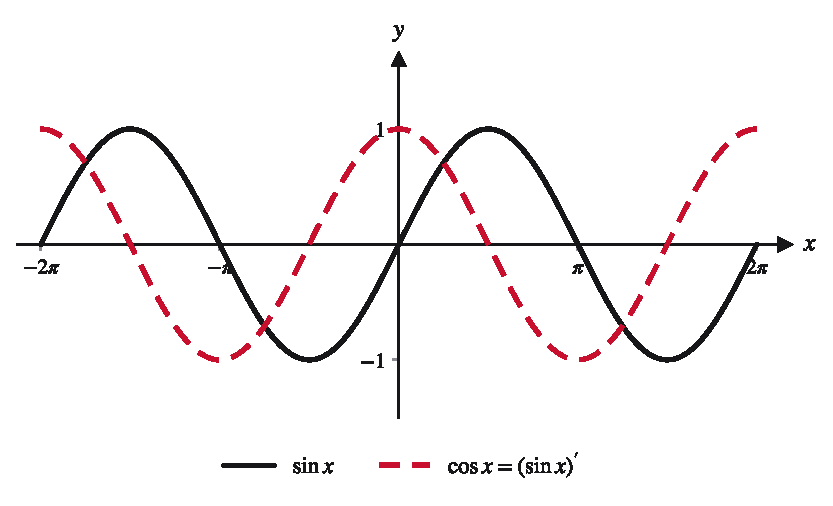
\includegraphics[width=400pt]{fig/m01_f02.pdf}
\caption{Les funcions $\sin x$ i $\cos x = (\sin x)'$ il\textperiodcentered{}lustren la seqüència cíclica de derivades successives de les funcions trigonomètriques.}
\end{figure}

\section{Taula de derivades}

La taula següent recull les derivades de les funcions elementals més habituals, on $u = u(x)$ denota una funció derivable genèrica i $u' = u'(x)$ la seva derivada.

\begin{table}[!htbp]
\centering
\renewcommand{\arraystretch}{1.75}
\begin{tabular}{lccc}
\toprule
Funció & Derivada & Funció & Derivada \\
\midrule
$k$ & $0$ & $\arctan u$ & $\displaystyle \dfrac{u'}{1+u^2}$ \\
$ax$ & $a$ & $\operatorname{arcsec} u$ & $\displaystyle \dfrac{u'}{u\sqrt{u^2-1}}$ \\
$u^n$ & $n\,u^{n-1}u'$ & $\operatorname{arccosec} u$ & $\displaystyle -\dfrac{u'}{u\sqrt{u^2-1}}$ \\
$\sqrt{u}$ & $\displaystyle \dfrac{u'}{2\sqrt{u}}$ & $\operatorname{arccotg} u$ & $\displaystyle -\dfrac{u'}{1+u^2}$ \\
$\sqrt[n]{u}$ & $\displaystyle \dfrac{u'}{n\sqrt[n]{u^{n-1}}}$ & $\sinh u$ & $\cosh u\cdot u'$ \\
$e^u$ & $e^u u'$ & $\cosh u$ & $\sinh u\cdot u'$ \\
$a^u$ & $a^u\ln a\cdot u'$ & $\tanh u$ & $\displaystyle \dfrac{u'}{\cosh^2 u}$ \\
$\ln u$ & $\displaystyle \dfrac{u'}{u}$ & $\operatorname{sech} u$ & $-\operatorname{sech} u\tanh u\cdot u'$ \\
$\log_a u$ & $\displaystyle \dfrac{u'}{u\ln a}$ & $\operatorname{cosech} u$ & $-\operatorname{cosech} u\coth u\cdot u'$ \\
$\sin u$ & $\cos u\cdot u'$ & $\coth u$ & $-\operatorname{cosech}^2 u\cdot u'$ \\
$\cos u$ & $-\sin u\cdot u'$ & $\operatorname{arcsinh} u$ & $\displaystyle \dfrac{u'}{\sqrt{u^2+1}}$ \\
$\tan u$ & $\displaystyle \dfrac{u'}{\cos^2 u}$ & $\operatorname{arccosh} u$ & $\displaystyle \dfrac{u'}{\sqrt{u^2-1}}$ \\
$\sec u$ & $\displaystyle \dfrac{u'\sin u}{\cos^2 u}$ & $\operatorname{arctanh} u$ & $\displaystyle \dfrac{u'}{1-u^2}$ \\
$\csc u$ & $\displaystyle -\dfrac{u'\cos u}{\sin^2 u}$ & $\operatorname{arcsech} u$ & $\displaystyle -\dfrac{u'}{u\sqrt{1-u^2}}$ \\
$\cot u$ & $\displaystyle -\dfrac{u'}{\sin^2 u}$ & $\operatorname{arccsch} u$ & $\displaystyle -\dfrac{u'}{u\sqrt{1+u^2}}$ \\
$\arcsin u$ & $\displaystyle \dfrac{u'}{\sqrt{1-u^2}}$ & $\operatorname{arccoth} u$ & $\displaystyle \dfrac{u'}{1-u^2}$ \\
$\arccos u$ & $\displaystyle -\dfrac{u'}{\sqrt{1-u^2}}$ &  &  \\
\bottomrule
\end{tabular}
\end{table}

\textbf{Operacions amb derivades}

\begin{table}[!htbp]
\centering
\renewcommand{\arraystretch}{1.75}
\begin{tabular}{lccc}
\toprule
Funció & Derivada & Funció & Derivada \\
\midrule
$k\cdot u$ & $k\cdot u'$ & $u+v-w$ & $u'+v'-w'$ \\
$\displaystyle \dfrac{k}{u}$ & $\displaystyle -\dfrac{k\,u'}{u^2}$ & $u\cdot v$ & $u'v+uv'$ \\
$u+v$ & $u'+v'$ & $\displaystyle \dfrac{u}{v}$ & $\displaystyle \dfrac{u'v-uv'}{v^2}$ \\
$u-v$ & $u'-v'$ &  &  \\
\bottomrule
\end{tabular}
\end{table}

\section{Complement: recta tangent i recta normal a una corba}

Geomètricament, $f'(a)$ és el \textbf{pendent de la recta tangent} a la gràfica de $f$ en el punt $P(a, f(a))$. Amb això es poden escriure les equacions de les dues rectes més demanades en un problema de derivades.

\textbf{Propietat (Recta tangent i recta normal):} si $f$ és derivable en $x=a$:

\begin{itemize}
\item \textbf{Tangent:} $\;y - f(a) = f'(a)\,(x - a)$
\item \textbf{Normal} (perpendicular a la tangent), si $f'(a)\neq 0$: $\;y - f(a) = -\dfrac{1}{f'(a)}\,(x - a)$
\end{itemize}

Si $f'(a) = 0$, la tangent és horitzontal ($y = f(a)$) i la normal és la recta vertical $x = a$.

\subsection{Mètode}

\begin{enumerate}
\item Calcular $f(a)$: això dona el punt $P(a, f(a))$.
\item Derivar $f$ i calcular el pendent $m = f'(a)$.
\item Escriure la tangent amb la fórmula punt-pendent. El pendent de la normal és $-1/m$.
\item Aïllar $y$ per donar l'equació en forma explícita.
\end{enumerate}

\subsection{Exemple 1 --- Tangent i normal en un punt}

Trobeu la tangent i la normal a $f(x) = x^2 - 3x + 2$ en $x = 3$.

\begin{itemize}
\item $f(3) = 9 - 9 + 2 = 2$, per tant $P(3, 2)$.
\item $f'(x) = 2x - 3 \Rightarrow m = f'(3) = 3$.
\item \textbf{Tangent:} $y - 2 = 3(x - 3) \Rightarrow y = 3x - 7$.
\item \textbf{Normal:} $y - 2 = -\dfrac13 (x - 3) \Rightarrow y = -\dfrac{x}{3} + 3$.
\end{itemize}

\begin{figure}[!htbp]
\centering
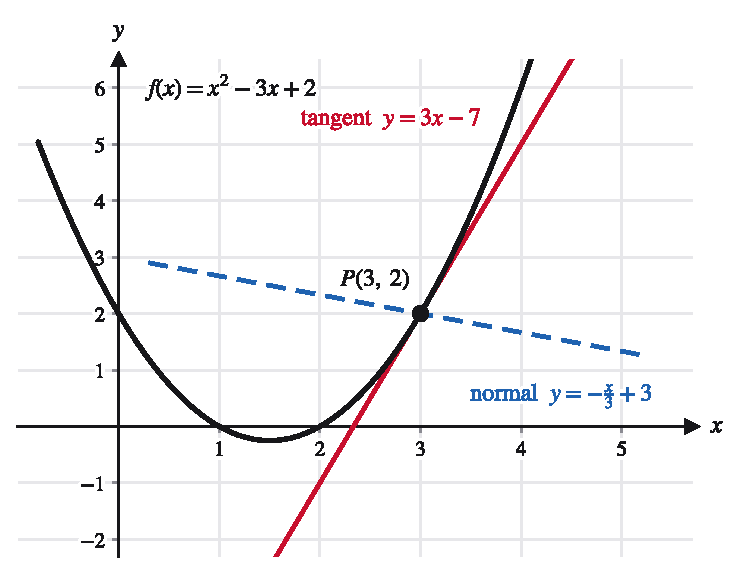
\includegraphics[width=356pt]{fig/m01_f28.pdf}
\caption{Tangent (vermell) i normal (blau, discontínua) a $f(x) = x^2 - 3x + 2$ en el punt $P(3, 2)$.}
\end{figure}

\subsection{Exemple 2 --- Tangents amb un pendent donat}

En quins punts de $f(x) = x^3 - 3x$ la tangent és paral\textperiodcentered{}lela a la recta $y = 9x + 1$?

Dues rectes són paral\textperiodcentered{}leles si tenen el mateix pendent: cal $f'(x) = 9$.

\begin{equation*}
f'(x) = 3x^2 - 3 = 9 \;\Rightarrow\; x^2 = 4 \;\Rightarrow\; x = \pm 2
\end{equation*}

\begin{itemize}
\item En $x = 2$: $f(2) = 2$, tangent $y - 2 = 9(x - 2) \Rightarrow y = 9x - 16$.
\item En $x = -2$: $f(-2) = -2$, tangent $y + 2 = 9(x + 2) \Rightarrow y = 9x + 16$.
\end{itemize}

\emph{Idea clau:} si l'enunciat dona una condició sobre la tangent (horitzontal, paral\textperiodcentered{}lela a una recta, perpendicular a una recta), s'imposa sobre $f'(x)$ i es resol l'equació.

\section{Complement: interpretació geomètrica i física de la derivada}

Quan $h$ tendeix a $0$, el punt $Q=(a+h,f(a+h))$ s'acosta a $P=(a,f(a))$ i la recta secant $PQ$ tendeix a la \textbf{recta tangent} a la corba en $P$. El pendent de la secant és la variació mitjana $\dfrac{f(a+h)-f(a)}{h}$ i el de la tangent és el seu límit, és a dir, $f'(a)$.

\begin{figure}[!htbp]
\centering
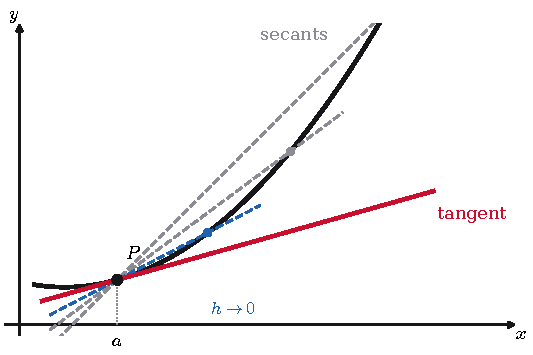
\includegraphics[width=256pt]{fig/x01_secant_tangent.pdf}
\caption{Les rectes secants (discontínues) s'aproximen a la recta tangent (vermell) quan $h\to0$: el pendent de la tangent és $f'(a)$.}
\end{figure}

La mateixa idea té una lectura física. Si $s(t)$ és la posició d'un mòbil en funció del temps, aleshores

\begin{equation*}
v(t)=s'(t)\ \text{(velocitat instantània)},\qquad a(t)=v'(t)=s''(t)\ \text{(acceleració)}.
\end{equation*}

Més generalment, $f'(a)$ mesura la \textbf{taxa de variació instantània} de $f$ en $x=a$: quant canvia $f$ per cada unitat que canvia $x$.

\emph{Exemple:} Un mòbil es mou segons $s(t)=t^3-6t^2+9t$ (metres, segons). Aleshores $v(t)=3t^2-12t+9=3(t-1)(t-3)$ i $a(t)=6t-12$. El mòbil s'atura ($v=0$) en $t=1$ s i $t=3$ s; en $t=1$ és a $s(1)=4$ m i en $t=3$ és a $s(3)=0$ m. Entre $t=1$ i $t=3$ la velocitat és negativa: retrocedeix.

\section{Complement: derivades laterals i punts de no derivabilitat}

\textbf{Definició:} Les \textbf{derivades laterals} de $f$ en $x=a$ són

\begin{equation}
f'(a^{+})=\lim_{h\to0^{+}}\frac{f(a+h)-f(a)}{h},\qquad f'(a^{-})=\lim_{h\to0^{-}}\frac{f(a+h)-f(a)}{h}.
\end{equation}

\textbf{Propietat:} $f$ és derivable en $x=a$ si i només si existeixen $f'(a^{+})$ i $f'(a^{-})$, són finites i són iguals. Aleshores $f'(a)=f'(a^{+})=f'(a^{-})$.

Una funció contínua pot deixar de ser derivable en un punt de tres maneres:

\begin{itemize}
\item \textbf{Punt angulós:} les derivades laterals existeixen però són diferents (exemple: $f(x)=|x|$ en $x=0$, amb $f'(0^-)=-1$ i $f'(0^+)=1$).
\item \textbf{Punt cuspidal:} les derivades laterals són infinites de signe oposat (exemple: $f(x)=x^{2/3}$ en $x=0$).
\item \textbf{Tangent vertical:} les dues derivades laterals són $+\infty$ (o $-\infty$) (exemple: $f(x)=\sqrt[3]{x}$ en $x=0$).
\end{itemize}

\begin{figure}[!htbp]
\centering
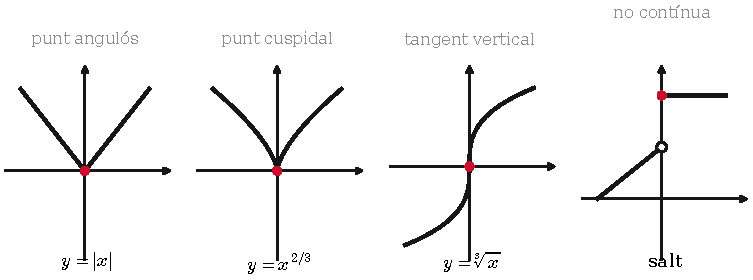
\includegraphics[width=361pt]{fig/x01_nonderiv.pdf}
\caption{Punts de no derivabilitat d'una funció contínua (punt angulós, cuspidal i tangent vertical) i funció no contínua (salt), que tampoc no és derivable.}
\end{figure}

\emph{Exemple:} Estudiem la derivabilitat de $f(x)=\begin{cases}x^2 & x\le1\\ 2x-1 & x>1\end{cases}$ en $x=1$. Contínua: $f(1^-)=1=f(1^+)$. Derivades laterals: $f'(1^-)=2x\big|_{x=1}=2$ i $f'(1^+)=2$. Coincideixen, per tant $f$ és derivable en $x=1$ amb $f'(1)=2$ (la recta $y=2x-1$ és tangent a la paràbola en $(1,1)$).

\section{Complement: demostració de les regles bàsiques de derivació}

\emph{Demostració de la derivada d'un producte.} Per a $h(x)=u(x)\,v(x)$,

\begin{equation*}
h'(x)=\lim_{h\to0}\frac{u(x+h)v(x+h)-u(x)v(x)}{h}=\lim_{h\to0}\Bigl[\frac{u(x+h)-u(x)}{h}\,v(x+h)+u(x)\,\frac{v(x+h)-v(x)}{h}\Bigr].
\end{equation*}

Com que $v$ és contínua, $v(x+h)\to v(x)$ i s'obté $(uv)'=u'v+uv'$. $\blacksquare$

\emph{Demostració de la derivada d'un quocient.} Si $q=\dfrac uv$, aleshores $u=q\,v$ i, derivant, $u'=q'v+qv'$. Aïllant, $q'=\dfrac{u'-qv'}{v}=\dfrac{u'v-uv'}{v^{2}}$. $\blacksquare$

\emph{Demostració de $(\sin x)'=\cos x$.} Amb la fórmula del sinus de la suma i els límits notables $\lim\limits_{h\to0}\frac{\sin h}{h}=1$ i $\lim\limits_{h\to0}\frac{\cos h-1}{h}=0$:

\begin{equation*}
(\sin x)'=\lim_{h\to0}\frac{\sin x\cos h+\cos x\sin h-\sin x}{h}=\sin x\cdot0+\cos x\cdot1=\cos x.\ \blacksquare
\end{equation*}

\emph{Demostració de $(x^n)'=n\,x^{n-1}$ ($n$ natural).} Pel binomi de Newton, $(x+h)^n=x^n+n\,x^{n-1}h+\binom n2x^{n-2}h^2+\dots+h^n$, de manera que $\dfrac{(x+h)^n-x^n}{h}=n\,x^{n-1}+h\,(\dots)\to n\,x^{n-1}$. $\blacksquare$

\section{Complement: derivació logarítmica, implícita, paramètrica i funció inversa}

\textbf{Derivació logarítmica.} Per a funcions del tipus $y=f(x)^{g(x)}$ es prenen logaritmes: $\ln y=g(x)\ln f(x)$, es deriva i s'aïlla $y'$:

\begin{equation*}
\frac{y'}{y}=g'\ln f+g\,\frac{f'}{f}\ \Longrightarrow\ y'=f^{\,g}\Bigl(g'\ln f+g\,\frac{f'}{f}\Bigr).
\end{equation*}

\emph{Exemple:} $y=x^{x}$ ($x>0$). $\ln y=x\ln x\Rightarrow\dfrac{y'}{y}=\ln x+1\Rightarrow y'=x^{x}(\ln x+1)$.

\textbf{Derivació implícita.} Si $y$ ve donada per una equació $F(x,y)=0$, es deriva respecte de $x$ considerant $y=y(x)$ i s'aïlla $y'$. \emph{Exemple:} a la circumferència $x^2+y^2=25$, derivant $2x+2y\,y'=0\Rightarrow y'=-\dfrac xy$. En el punt $(3,4)$ el pendent és $-\dfrac34$ i la tangent és $y-4=-\dfrac34(x-3)$, és a dir, $3x+4y=25$.

\textbf{Derivació paramètrica.} Si $x=x(t)$, $y=y(t)$, aleshores $\dfrac{dy}{dx}=\dfrac{y'(t)}{x'(t)}$. \emph{Exemple:} $x=t^2$, $y=t^3$: $\dfrac{dy}{dx}=\dfrac{3t^2}{2t}=\dfrac{3t}{2}$.

\textbf{Derivada de la funció inversa.} Si $f$ és derivable i bijectiva amb $f'(x)\neq0$, aleshores $(f^{-1})'(y)=\dfrac{1}{f'(x)}$ amb $y=f(x)$. \emph{Exemple:} $f(x)=x^3+x$ és creixent i $f(1)=2$, per tant $(f^{-1})'(2)=\dfrac{1}{f'(1)}=\dfrac14$. Aquesta regla permet deduir, per exemple, $(\arctan x)'=\dfrac{1}{1+x^2}$ a partir de $(\tan y)'=1+\tan^2y$.

\section{Complement: exemples resolts de derivades}

a) $f(x)=x^2e^{3x}$. Producte: $f'(x)=2x\,e^{3x}+x^2\cdot3e^{3x}=x\,e^{3x}(2+3x)$.

b) $f(x)=\ln(x^2+1)$. Regla de la cadena: $f'(x)=\dfrac{2x}{x^2+1}$.

c) $f(x)=\sin(x^2)\cos x$. $f'(x)=2x\cos(x^2)\cos x-\sin(x^2)\sin x$.

d) $f(x)=\dfrac{2x+1}{x^2-3}$. Quocient: $f'(x)=\dfrac{2(x^2-3)-(2x+1)2x}{(x^2-3)^2}=\dfrac{-2(x^2+x+3)}{(x^2-3)^2}$.

e) $f(x)=\sqrt{1+x^2}$. $f'(x)=\dfrac{2x}{2\sqrt{1+x^2}}=\dfrac{x}{\sqrt{1+x^2}}$.

f) $f(x)=\arctan\sqrt x$. Amb $u=\sqrt x$, $u'=\dfrac1{2\sqrt x}$: $f'(x)=\dfrac{1}{1+x}\cdot\dfrac{1}{2\sqrt x}=\dfrac{1}{2\sqrt x\,(1+x)}$.

g) $f(x)=\dfrac{\ln x}{x}$. $f'(x)=\dfrac{\frac1x\cdot x-\ln x}{x^2}=\dfrac{1-\ln x}{x^2}$.

h) $f(x)=e^{\sin x}$. $f'(x)=\cos x\,e^{\sin x}$.

\emph{Comprovació:} una bona pràctica és verificar el resultat amb un valor concret, per exemple $f(x)=x^2e^{3x}$ en $x=0$: $f'(0)=0$, coherent amb $x\,e^{3x}(2+3x)=0$.
